% ============================================================
%  P3 — Applied Machine Learning: BiasBios
%  module_summary.tex  |  Machine Learning Analysis Report
% ============================================================

\documentclass[11pt, a4paper]{article}

\usepackage[margin=2.5cm]{geometry}
\usepackage{setspace}
\usepackage{parskip}
\usepackage{hyperref}
\usepackage{booktabs}
\usepackage{graphicx}
\usepackage{amsmath}
\usepackage{natbib}
\usepackage{microtype}

\title{%
    \textbf{Machine Learning Analysis Report} \\[0.4em]
    \large Occupation Classification and Gender Bias in Professional Biographies
}
\author{Stefan Ohms}
\date{\today}

% ============================================================
\begin{document}
\maketitle
\tableofcontents
\newpage

\section{Overview}

This project trains a 28-class occupation classifier on professional biography 
text using the BiasBios dataset \citep{de2019bias}, as reconstructed and released 
by \citet{ravfogel2020null} and hosted on Hugging Face \citep{labHC_bias_in_bios}. 
Logistic regression was chosen because its weight matrix is directly readable as 
a mechanism: inspecting it requires no separate probe or approximation. 
Weight inspection revealed gender signal concentrated in a small number of 
features, enabling a targeted intervention: removing nine pronoun tokens reduced 
mean gender correlation by 40\% at no cost to macro F1. 
This interpretability is a consequence of model capacity rather than deliberate 
design, and its limits as complexity grows are the central question of the 
broader project arc.

\section{Dataset Description}

\citet{de2019bias} compiled a dataset of professional biographies, along with 
their occupations and genders, from a web crawl. Although the crawling code was 
released, the dataset itself was not. \citet{ravfogel2020null} released a 
reconstructed version for their own experiments, which is the version used here, 
hosted on Hugging Face by Laboratoire Hubert Curien \citep{labHC_bias_in_bios}. 
The reconstructed version contains 396,189 biographies across 28 occupation 
classes, slightly smaller than the original due to 5,557 biographies no longer 
available on OpenCrawl at the time of reconstruction.

The dataset contains four columns: \texttt{hard\_text} (biography text), 
\texttt{profession} (integer-encoded occupation class), \texttt{gender} 
(binary integer: 0 for male, 1 for female), and \texttt{split} 
(train, dev, or test). The predefined splits from \citet{ravfogel2020null} 
are preserved exactly: 257,478 biographies in train, 39,642 in dev, and 
99,069 in test. The dev set is used for hyperparameter tuning and the test 
set is held out until final evaluation. The \texttt{gender} column is not 
used as a model input; it is retained exclusively for the ethics analysis. 
Although integer encoding aids training, it hampers interpretation: two 
columns were added during preprocessing, \texttt{profession\_text} and 
\texttt{gender\_text}, containing the corresponding textual labels for each 
integer code.

\section{Modeling Approach}

The modeling pipeline begins with feature engineering. Biographies are 
converted to numerical vectors using TF-IDF, the standard bag-of-words 
vectorisation method in classical NLP \citep{schutze2008introduction}. 
Compared to raw count vectors, TF-IDF's IDF weighting suppresses terms 
common across documents while sublinear TF normalisation reduces the 
dominance of high-frequency terms, making it strictly preferable for text 
classification. The vocabulary is restricted to terms appearing in at least 
0.1\% and at most 99\% of documents, yielding 4,402 active features after 
filtering. Stopword removal is deliberately skipped to preserve explicit 
gender indicators such as \textit{he} and \textit{she}, which are central 
to the ethics analysis. The vectoriser is fitted on the training set only 
to prevent data leakage.

Logistic regression was chosen as the classifier. Beyond its computational 
efficiency, its coefficient matrix is directly readable as a mechanism: 
each weight encodes the contribution of a single feature to a single class 
prediction, requiring no post-hoc approximation to interpret. This makes 
logistic regression the degenerate case of a linear probe 
\citep{alain2016understanding}, where the probe and the model are identical. 
However, this interpretability is a consequence of the model's limited 
capacity: the same linearity that makes the weights readable also bounds 
expressiveness, and performance on most tasks falls short of modern deep 
learning.

The only hyperparameter requiring tuning is C, the inverse regularisation 
strength, which directly controls the bias-variance tradeoff and is 
sensitive to feature space scale \citep{hastie2009elements}. A grid search 
over candidate values was conducted, scoring on macro-averaged F1 to weight 
all 28 classes equally regardless of size. To avoid overfitting to the test 
set, tuning used the predefined dev split from \citet{ravfogel2020null} via 
\texttt{PredefinedSplit}. The search identified $C = 1.0$ as optimal. The 
model was trained using the L-BFGS solver for up to 1,000 iterations with 
balanced class weighting, which adjusts loss contributions inversely 
proportional to class frequency. Given the strong overrepresentation of 
professors (29,520 test examples vs.\ 351 for rapper), balanced weighting 
prevents the model from defaulting to majority-class predictions at the 
expense of rarer occupations.

A \texttt{DummyClassifier} predicting the most frequent class at all times 
serves as the baseline, yielding a macro F1 of 0.02 and an accuracy of 30\%. 
This establishes the floor against which the logistic regression model is 
evaluated.

\section{Results}

The logistic regression model achieves 76\% accuracy and a macro-averaged 
F1 of 0.68 on the test set, compared to the majority-class baseline accuracy 
of 30\% and macro F1 of 0.02. The improvement of 0.66 macro F1 points 
demonstrates that the model has learned meaningful discriminative features 
across professions rather than exploiting class imbalance.

Macro-averaged F1 is the primary evaluation metric, weighting all 28 classes 
equally regardless of size. Accuracy alone would be misleading given the 
strong overrepresentation of professors (29,520 test examples). 
Table~\ref{tab:results_summary} summarises the overall results and 
Table~\ref{tab:results_per_class} highlights the best and worst performing 
classes.

\begin{table}[h]
\centering
\begin{tabular}{lcc}
\hline
\textbf{Model} & \textbf{Accuracy} & \textbf{Macro F1} \\
\hline
DummyClassifier (most frequent) & 0.30 & 0.02 \\
Logistic Regression             & 0.76 & 0.68 \\
\hline
\end{tabular}
\caption{Classification performance on the test set (n = 99,069).}
\label{tab:results_summary}
\end{table}

\begin{table}[h]
\centering
\begin{tabular}{lcccc}
\hline
\textbf{Profession} & \textbf{Precision} & \textbf{Recall} & 
\textbf{F1} & \textbf{Support} \\
\hline
dentist            & 0.93 & 0.92 & 0.93 & 3{,}647 \\
attorney           & 0.89 & 0.83 & 0.86 & 8{,}143 \\
photographer       & 0.89 & 0.80 & 0.85 & 6{,}068 \\
nurse              & 0.81 & 0.83 & 0.82 & 4{,}738 \\
\hline
pastor             & 0.31 & 0.74 & 0.44 &   632 \\
interior\_designer & 0.37 & 0.73 & 0.49 &   366 \\
paralegal          & 0.45 & 0.75 & 0.56 &   442 \\
\hline
\end{tabular}
\caption{Best and worst performing classes on the test set.}
\label{tab:results_per_class}
\end{table}

The best performing classes all have distinctive occupational vocabulary. 
The weakest class is pastor (F1 = 0.44), a surprising result given that 
clerical biographies might be expected to contain relatively distinctive 
language. Interior designer (0.49) and paralegal (0.56) likely suffer from 
vocabulary overlap with adjacent professions. The consistent recall scores 
across classes confirm that balanced class weighting is effective at 
preventing majority-class dominance.

\section{Ethics, Interpretability and Bias}

In mechanistic interpretability, linear probes are trained on top of a 
model's internal representations to test what information is encoded at a 
given layer \citep{alain2016understanding}. The probe is a separate, 
lightweight classifier layered on top of an opaque model to recover what 
the model itself cannot explain. Logistic regression does not require this 
indirection. The weight matrix directly maps TF-IDF features to class 
predictions, meaning the model's decision logic is fully exposed without 
any additional machinery. This is not a deliberate design choice for 
interpretability; it is a consequence of the model's limited capacity. 
The same linearity that constrains expressiveness makes the internal logic 
directly readable: the weights are the probe.

The model has learned 4,402 weights for each of the 28 professions, 
expressed as the softmax function:

$$P(y = k \mid \mathbf{x}) = \frac{e^{\mathbf{w}_k \cdot \mathbf{x} + 
b_k}}{\sum_{j=1}^{K} e^{\mathbf{w}_j \cdot \mathbf{x} + b_j}}$$

This is the same output layer used in modern neural classifiers. A feature 
drives a prediction when two conditions hold: its weight is large, and its 
presence in the input is strong. The relevant quantity is therefore the 
logit contribution, the product of weight and input signal strength, rather 
than the weight alone.

The top 25 features by weight are extracted per occupation class and their 
logit contributions are correlated with the binary gender label using the 
point-biserial correlation coefficient \citep{lev1949point}, the appropriate 
statistic when one variable is continuous and the other is binary, 
mathematically equivalent to Pearson's $r$ in this case. The sign is 
directly interpretable: positive values indicate female-correlated features, 
negative values indicate male-correlated features. \citet{de2019bias} 
identified gender bias in this dataset; the weight inspection here confirms 
and localises it.

As shown in Figure~\ref{fig:bias_corr_0}, the pattern is strikingly 
symmetric: \textit{she} dominates female-correlated professions including 
dietitian, nurse, yoga\_teacher, model, and teacher, while \textit{he} 
dominates male-correlated professions including chiropractor, surgeon, 
software\_engineer, comedian, and pastor, both at absolute correlations of 
approximately 0.75. In the middle tier, occupation-specific terms such as 
\textit{nursing}, \textit{dr}, and \textit{software} dominate, suggesting 
the model relies on occupational vocabulary rather than gendered pronouns 
for these classes. Figure~\ref{fig:bias_corr_1} confirms that gender signal 
is concentrated in pronouns rather than distributed across the weight 
vector: correlations drop sharply at the second-ranked feature, where 
occupation-specific terms dominate instead.

\begin{figure}[h]
    \centering
    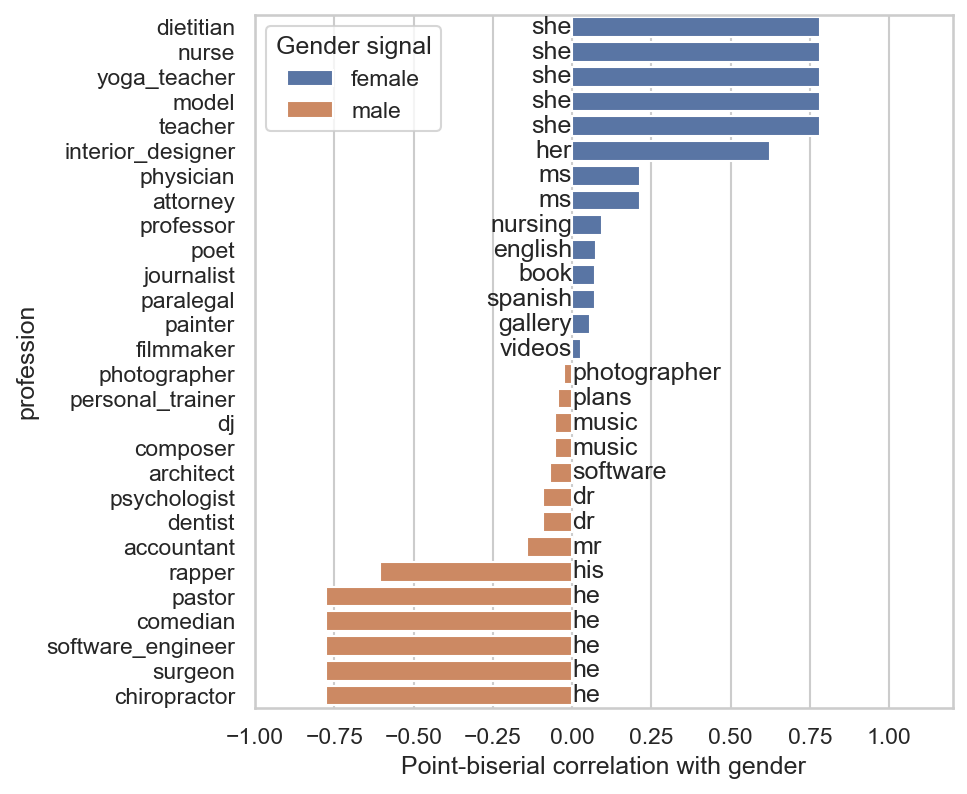
\includegraphics[width=0.85\textwidth]{figures/gender_bias_correlation_0.png}
    \caption{Top-ranked gender-correlated feature per profession in the 
    baseline model. Bar width indicates point-biserial correlation strength; 
    colour indicates direction (female/male). Feature name is displayed next 
    to each bar.}
    \label{fig:bias_corr_0}
\end{figure}

\begin{figure}[h]
    \centering
    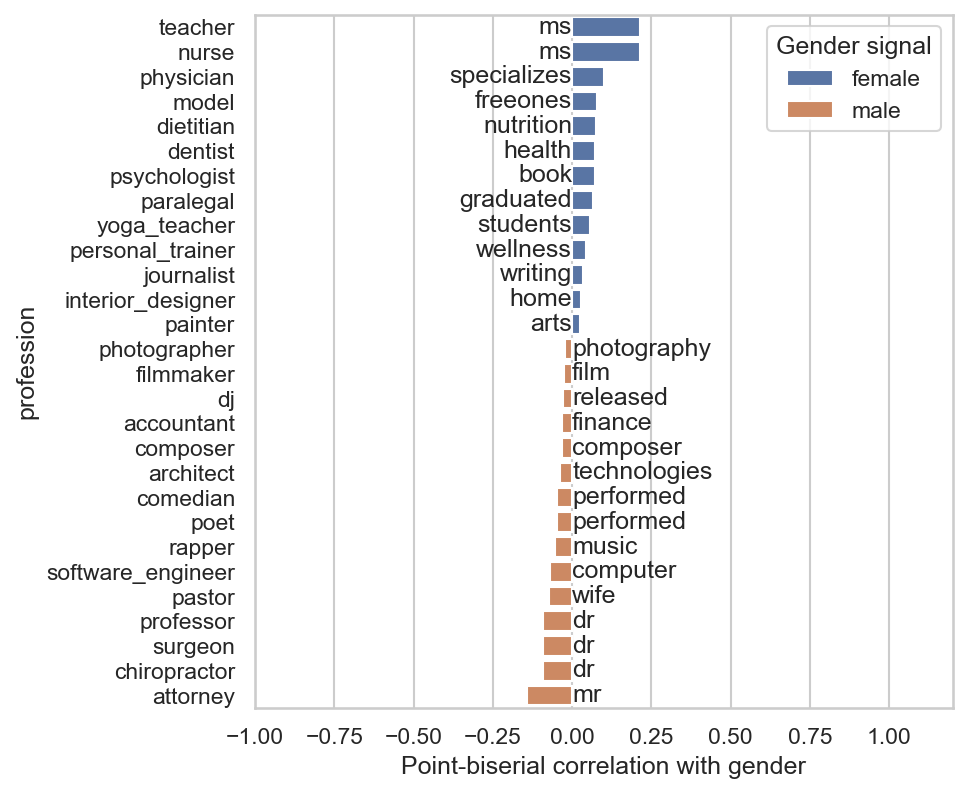
\includegraphics[width=0.85\textwidth]{figures/gender_bias_correlation_1.png}
    \caption{Second-ranked gender-correlated feature per profession in the 
    baseline model. Correlations drop sharply relative to 
    Figure~\ref{fig:bias_corr_0}, confirming that gender signal is 
    concentrated rather than distributed.}
    \label{fig:bias_corr_1}
\end{figure}

This localisation enables a targeted intervention. A pronoun stop list of 
nine tokens (\textit{she, her, hers, he, his, him, ms, mr, mrs}) is added 
to the TF-IDF vectoriser, with all other hyperparameters held constant. 
Non-binary pronouns (\textit{they, them, their}) are deliberately excluded 
as they are common in generic English usage. The two models are compared on 
macro F1 and on mean absolute point-biserial correlation, defined as:

$$\bar{r} = \frac{1}{C}\sum_{c=1}^{C}\frac{1}{K}\sum_{k=1}^{K}|r_{c,k}|$$

where $C = 28$ occupation classes, $K = 25$ top-weighted features per 
class, and $r_{c,k}$ is the point-biserial correlation between the logit 
contribution of feature $k$ in class $c$ and the binary gender label.

The intervened model achieves a macro F1 of 0.68, identical to the 
baseline, confirming that occupational predictive signal is carried by 
content vocabulary rather than gendered pronouns. Mean $\bar{r}$ falls 
from 0.035 to 0.021, a reduction of 40\%, as shown in 
Figure~\ref{fig:bias_comparison}. Residual gendered signal remains: 
\textit{wife} and \textit{husband} appear as top features in the intervened 
model, indicating that gendered language extends beyond explicit pronouns. 
A more complete debiasing would require suppressing gender information 
directly in the representation space, an approach that becomes necessary 
as model complexity grows and the weight matrix is no longer directly 
readable.

\begin{figure}[h]
    \centering
    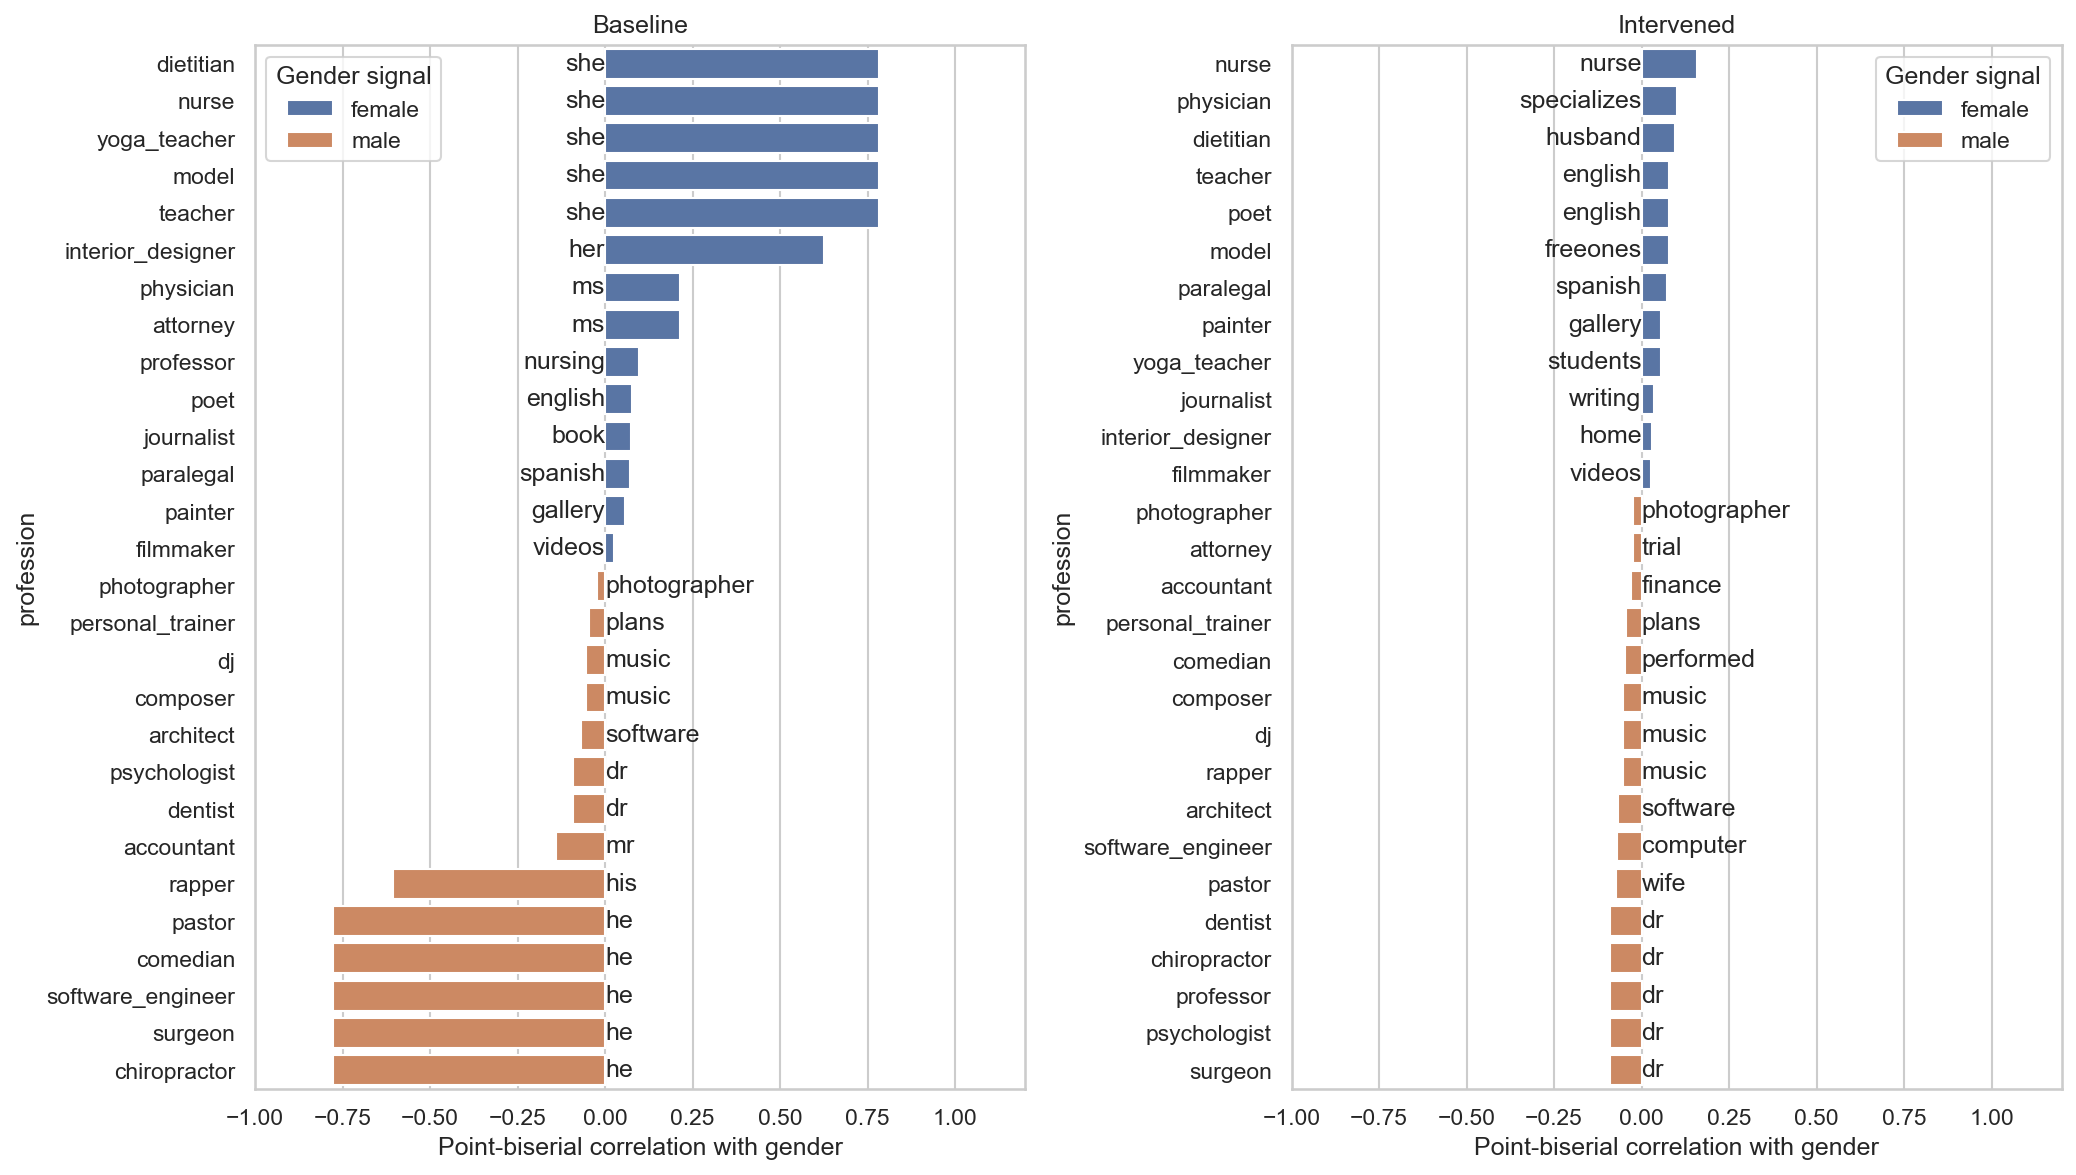
\includegraphics[width=\textwidth]{figures/gender_bias_comparison.png}
    \caption{Baseline (left) vs.\ intervened model (right): top-ranked 
    gender-correlated feature per profession. After removing nine pronoun 
    tokens, mean $\bar{r}$ falls from 0.035 to 0.021 (40\% reduction) 
    with no change in macro F1.}
    \label{fig:bias_comparison}
\end{figure}

Finally, it is worth acknowledging the researcher's own positionality. 
The framing of this analysis assumes that gender should not be 
determinative of professional classification. This is less an empirical 
claim than a moral and political conviction, and one that may not hold 
uniformly across cultural contexts. What is interpreted as bias here 
reflects a value judgment shared widely within the AI research community 
\citep{de2019bias}, but not universally. In the interest of the same 
transparency this project advocates for in models, it is worth making 
that assumption explicit: the reader should know the normative position 
from which the analysis proceeds.

\section{Interpretation for a Non-Technical Audience}

As the prevalence and capabilities of AI systems increase, our ability to 
understand what they are thinking and why they make their decisions is 
fading. Experts call the field that fights against this loss of 
interpretability Explainable AI. This analysis shows why understanding AI 
is of significant importance to its ethical employment.

The Bias in Bios dataset contains biographies compiled from the Internet, 
and its goal is to classify the profession of the person behind each 
biography. However, the dataset comes with a twist: it has a known gender 
bias and metadata indicating the biography's gender. The question is 
whether a machine learning model trained on this biased dataset will learn 
a gender bias towards certain professions. Should identifying gender matter 
when classifying someone as a model, a teacher, or a software engineer, or 
does this very act propagate stereotypes?

For the analysis, a classical machine learning model called logistic 
regression was trained. The reason is that it is easier to deduce the 
decision processes behind classical machine learning models than those of 
complex modern AI systems. What we found is a clear association of the word 
\textit{she} with nurses, teachers, models, dietitians, and yoga 
instructors. On the other hand, when \textit{he} is frequent in a 
biography, the model was more likely to assign professions such as 
chiropractor, surgeon, software engineer, comedian, or pastor. The bias 
present in the biographies was learned by the model.

The gendering of professions is a clear concern for perpetuating stereotypes 
that might reinforce patterns of a gendered society. An intervention was 
therefore conducted: pronouns were eliminated from the vocabulary fed into 
the model. This experiment showed that a model trained without pronouns was 
substantially less gender-biased than the original. What was surprising, 
however, was that its performance did not degrade. It was just as good at 
predicting professions as the more biased model.

What this shows is that there is a choice between training a gender-biased 
model and a far less gender-biased one, without sacrificing usability. 
Through the model's interpretability, it is sometimes possible to identify 
and reduce bias precisely. If we can find ways to apply this kind of 
analysis not just to simple classical models but also to modern AI systems, 
we may be able to make them more equitable. This idea will be explored 
further in subsequent projects.

\section{Limitations and Potential Bias}

The first limitation concerns the TF-IDF representation. As a bag-of-words 
method, it counts terms with frequency weighting but discards semantics, 
word order, and co-reference \citep{schutze2008introduction}. The pronoun 
\textit{she}, for example, may refer to the subject of the biography or to 
a third party mentioned in it, so the model cannot distinguish between these 
cases. Semantically richer representations such as learned word embeddings 
or transformer-based encoders would address this, but at the cost of the 
direct weight interpretability that this analysis depends on.

Second, the dataset originates from a web crawl and is known to 
over-represent academic biographies, with professors comprising 30\% of the 
test set \citep{de2019bias}. This sampling bias means the dataset does not 
represent the true distribution of professions in the population. A more 
representative dataset would require access to private documents such as 
CVs, which cannot be used in a reproducible academic setting. Subsampling 
or oversampling to better approximate the true distribution was out of scope 
for this project, given that the primary goal is to demonstrate how 
interpretability can expose and reduce bias rather than to maximise 
classification performance.

Third, the pronoun intervention is only partially effective. Tokens such as 
\textit{wife} and \textit{husband} survive the stop list and carry residual 
gender signal, confirming that gendered language is not limited to explicit 
pronouns. A more complete debiasing would require either a broader 
intervention or a method that suppresses gender information directly in the 
representation space.

Most fundamentally, the interpretability demonstrated here is a consequence 
of model capacity rather than a designed property \citep{alain2016understanding}. 
Logistic regression exposes its decision logic through the weight matrix 
because it has no intermediate representations. As model capacity grows 
from classical classifiers to recurrent networks to transformers, this 
direct readability breaks down: gender signal can be reconstructed from 
subtler co-occurring vocabulary even without explicit pronouns, and it 
becomes encoded in intermediate representations that are not directly 
readable. Recovering interpretability at higher capacity requires dedicated 
tools such as linear probes and sparse autoencoders. This is the central 
question the subsequent projects in this capstone arc address.

\section{Future Work}

This project demonstrates that interpretability is tractable at the level 
of logistic regression precisely because the model has no intermediate 
representations. The weight matrix is the mechanism, and reading it 
requires no additional tools. As model capacity grows, this property 
disappears.

Subsequent projects in this capstone arc investigate what happens at higher 
complexity. Recurrent networks and transformers encode information in 
intermediate representations that are not directly readable, and gender 
signal can be reconstructed from subtle co-occurring vocabulary even after 
explicit pronouns are removed. Recovering interpretability in these settings 
requires dedicated methods: linear probes \citep{alain2016understanding} to 
test what information is encoded at a given layer, and sparse autoencoders 
to recover monosemantic features from superposed representations. The 
question of whether bias can still be identified and reduced under these 
conditions, and at what cost, is the thread that connects this project to 
the rest of the arc.

\bibliographystyle{apalike}
\bibliography{references}

\end{document}